\subsection{Visión por computador}

La visión por computador es una disciplina de la inteligencia artificial que se dedica al desarrollo de algoritmos y sistemas capaces de interpretar y procesar visualmente la información contenida en imágenes digitales o secuencias de vídeo. Este campo multidisciplinario integra elementos de procesamiento de imágenes, aprendizaje automático, patrones de reconocimiento y percepción computacional, facilitando la extracción automática y el análisis detallado de datos visuales \cite{szeliski2022computer}.

Es aplicada actualmente en campos como la robótica avanzada, interfaces de realidad aumentada y virtual, sistemas de navegación autónoma, aplicaciones de vigilancia de seguridad y en la interfaz humano-computadora \cite{geron2019hands}.

Según expertos en el campo, como Patterson y Gibson \citeA{patterson2017deep}, esta área se divide esencialmente en dos subdominios: procesamiento de imágenes y reconocimiento de objetos. El primero se enfoca en la manipulación y mejora de datos visuales, mientras que el segundo se centra en la identificación e interpretación de entidades dentro de las imágenes.

\subsubsection{Clasificación y localización de objetos}

La clasificación de objetos implica la determinación del tipo de objeto presente en una imagen, una tarea que puede efectuarse sin necesidad de localizar su posición específica. Por ejemplo, la identificación de un perro en una imagen no requiere determinar su ubicación exacta \cite{szeliski2022computer}. En contraste, la localización de objetos se refiere a determinar la ubicación exacta de un objeto dentro de una imagen. Este proceso se asocia con técnicas de regresión, donde se predicen valores numéricos que representan la posición del objeto en el espacio visual \cite{geron2019hands}.

\subsubsection{Detección de objetos}

La detección de objetos combina las tareas de clasificación y localización, identificando y determinando la posición de múltiples objetos en una imagen. Este proceso se realiza mediante la generación de un cuadro delimitador (bounding box) que encierra cada objeto detectado, y la asignación de una etiqueta de clase a cada cuadro delimitador \cite{geron2019hands}, tal y como se muestra en la Figura~\ref{fig:object_detection}.

\begin{figure}[H]
    \begin{center}
        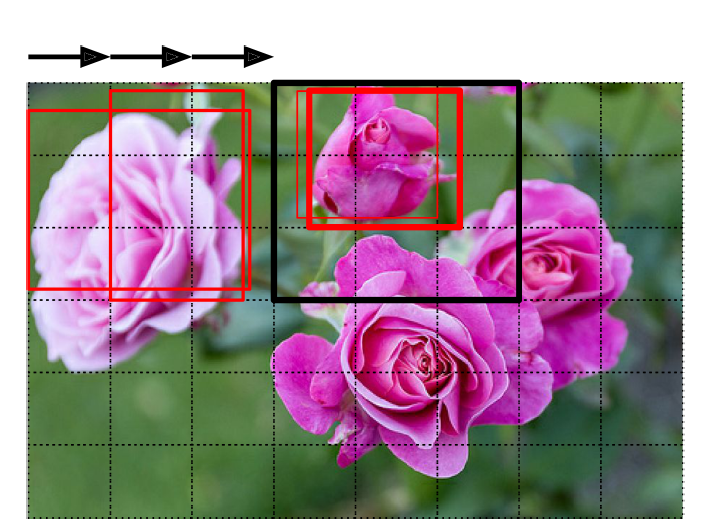
\includegraphics[width=0.6\textwidth]{Images/object_detection.png}
    \end{center}
    \caption{Detección de objetos.}
    \reference{Datos tomados de \citeA{geron2019hands}.}
    \label{fig:object_detection}
\end{figure}

\subsubsection{Segmentación semántica}

La segmentación semántica implica asignar una etiqueta específica a cada píxel de una imagen (ver Figura~\ref{fig:semantic_segmentation}). Esencialmente la segmentación semántica es una tarea de clasificación de píxeles, donde cada píxel de la imagen es clasificado en una categoría correspondiente \cite{patterson2017deep}

\begin{figure}[H]
    \begin{center}
        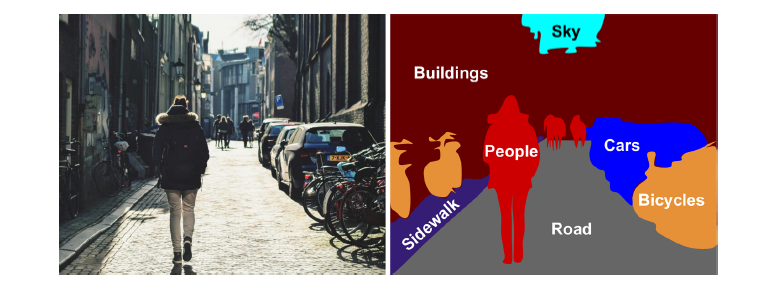
\includegraphics[width=1\textwidth]{Images/semantic_segmentation.png}
    \end{center}
    \caption{Segmentación semántica.}
    \reference{Datos tomados de \citeA{geron2019hands}.}
    \label{fig:semantic_segmentation}
\end{figure}

\subsubsection{Visión por computador empleando aprendizaje profundo}

La implementación de algoritmos de aprendizaje profundo en la resolución de problemas de visión por computador comprende varias etapas. Estas incluyen la preparación y preprocesamiento de datos, seguido por el desarrollo y afinamiento de modelos. Finalmente, se realiza la evaluación de estos modelos mediante la recolección y análisis de métricas de evaluación específicas.

\textbf{a) Conjunto de datos}

La asignación de los datos se realiza conforme a las proporciones determinadas por los requerimientos de la tarea en cuestión y por el estado del conocimiento actual en el área, para lo cual es esencial el uso de un conjunto de datos estructurado adecuadamente. Este conjunto se segmenta en tres subconjuntos esenciales: el de entrenamiento, el de validación y el de pruebas, como se establece en la Ecuación~\ref{equ:dataset}.

Dado un conjunto de datos \( X = \{(x_{0},y_{0}), ..., (x_{N},y_{N})\} \) que comprende \( N \) elementos, se puede definir \( x_{i} \) como la imagen en \( \mathbb{R}^{W \times H \times 3} \) y \( y_{i} \) como la categoría correspondiente, donde \( y_{i} \in \{1, ..., c\} \).

Se describe la partición del conjunto de datos como:

\begin{equation}
    \label{equ:dataset}
    X = X_{\text{train}} \cup X_{\text{val}} \cup X_{\text{test}}
\end{equation}

Es esencial mantener una exclusividad mutua entre los subconjuntos para preservar la validez de la evaluación, como lo indica la Ecuación~\ref{equ:dataset_interseccion}.

\begin{equation}
    \label{equ:dataset_interseccion}
    X_{\text{train}} \cap X_{\text{val}} = X_{\text{train}} \cap X_{\text{test}} = X_{\text{dev}} \cap X_{\text{test}} = \emptyset
\end{equation}

El subconjunto de entrenamiento se utiliza solo durante la fase de entrenamiento, y su rendimiento se evalúa intermitentemente con el subconjunto de validación. Después del entrenamiento, se realiza una evaluación del modelo usando el subconjunto de validación. Si el rendimiento es insuficiente, se deben hacer ajustes al modelo o considerar una nueva estrategia.

La evaluación final se lleva a cabo con el subconjunto de pruebas, en un procedimiento único que establecerá la efectividad del modelo en un contexto operativo real, como indican \citeA{aghdam2017guide}.

\subsubsection{Aumento de datos}

El aumento de datos es una técnica utilizada para mejorar la capacidad de generalización de los modelos de aprendizaje automático, en tareas de visión por computador. Consiste en la generación de nuevas instancias de entrenamiento a través de transformaciones que mantienen la esencia de los datos originales \cite{geron2019hands}. Estas transformaciones pueden incluir rotaciones, traslaciones, escalado, recorte, o cambios en la iluminación y color de las imágenes \cite{elgendy2020deep}.

\begin{figure}[H]
    \begin{center}
        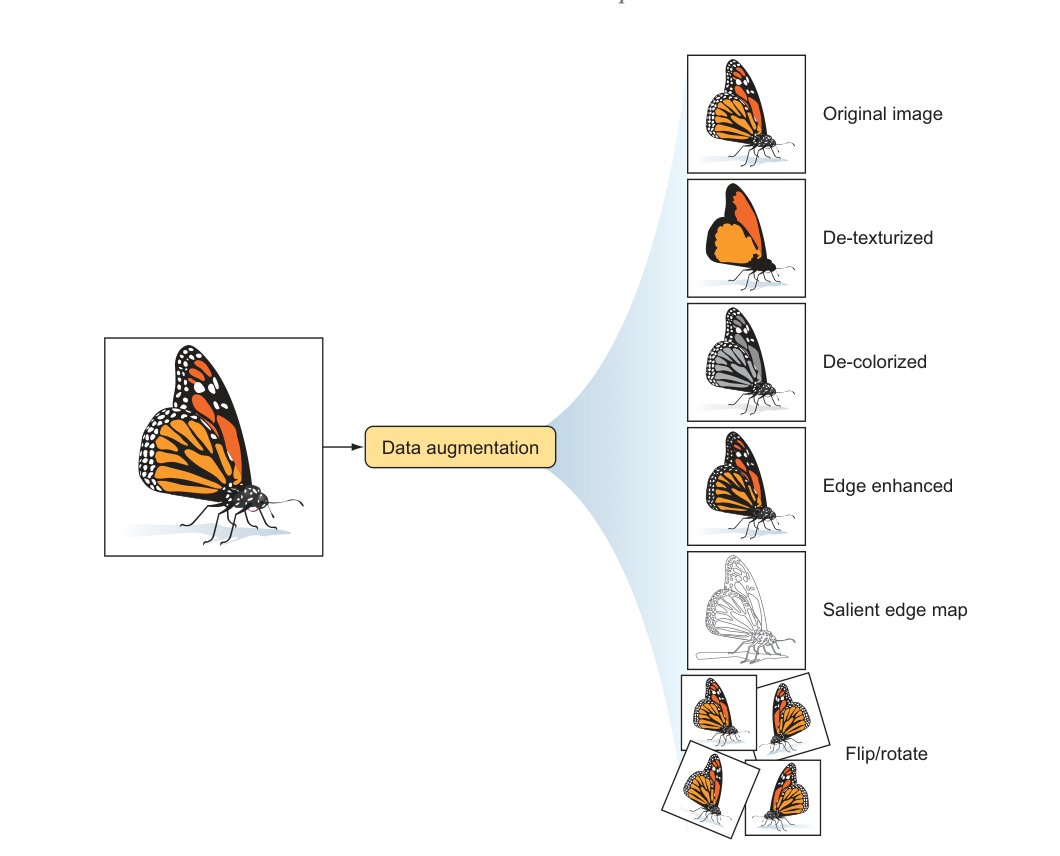
\includegraphics[width=0.8\textwidth]{Images/DataAumentation.png}
    \end{center}
    \caption{Transformaciones aplicadas en un proceso de aumento de datos.}
    \reference{Datos tomados de \citeA{elgendy2020deep}.}
    \label{fig:DataAumentation}
\end{figure}

La aplicación del aumento de datos se puede representar como una función de transformación \( T \) aplicada al conjunto de entrenamiento \( X_{\text{train}} \), generando un conjunto ampliado \( X'_{\text{train}} \) (ver Figura~\ref{fig:DataAumentation}).

\begin{equation}
    X'_{\text{train}} = \{ T(x) | x \in X_{\text{train}} \}
\end{equation}

Donde \( T \) representa una serie de operaciones de procesamiento de imágenes aleatorias o deterministas que se aplican a las imágenes \( x \) en \( X_{\text{train}} \).

Es fundamental que las transformaciones empleadas en el aumento de datos no alteren las etiquetas de clase de las imágenes, para que el modelo aprenda correctamente las características relevantes sin introducir ruido o ambigüedad \cite{aghdam2017guide}.

Autores, como \citeA{elgendy2020deep}, mencionan la importancia de establecer un equilibrio en la aplicación de estas técnicas para evitar el sobreajuste a transformaciones específicas que no sean relevantes para la tarea de clasificación o reconocimiento. La selección de las técnicas de aumento debe estar alineada con las características inherentes a las imágenes y la naturaleza de la tarea de aprendizaje automático.

En el contexto de la segmentación semántica, el aumento de datos debe preservar la información semántica de las categorías de objeto en las imágenes, y también la relación espacial entre los píxeles que componen cada objeto o región semántica \cite{aghdam2017guide}.

\subsubsection{Entrenamiento y validación}



\subsubsection{Métricas y evaluación de resultados}

La selección de las métricas adecuadas para la evaluación dependerá del tipo de tarea de visión por computador a resolver.

Para evaluar un modelo de clasificación de objetos, el resultado a analizar será únicamente la etiqueta resultante. En cambio, para evaluar un modelo de detección de objetos, no solo se analizará la etiqueta sino también el cuadro delimitador que identifica la ubicación y extensión del objeto en la imagen. En el caso de la segmentación semántica, donde el objetivo es clasificar cada píxel de una imagen en una categoría correspondiente, las métricas de evaluación deben reflejar la precisión de la asignación de píxeles a las categorías correctas \cite{patterson2017deep}.

\textbf{a) Accuracy}

Es una métrica de evaluación que calcula la fracción de muestras clasificadas correctamente. Por ejemplo, si se tiene $ {X}' = (x_{1},y_{1}), ... , (x_{N},y_{N})$ que representa un conjunto de datos de $N$ de elementos, la ecuación para obtener el accuracy correspondiente es la siguiente:

\begin{equation}
    accuracy = \frac{1}{N} \sum_{i=1}^{N} 1[y_{i} == \hat{y}_{i}]
\end{equation}

Donde, $ y_{i} $ y $ \hat{y}_{i} $ representan las etiquetas de verdad y las etiquetas predichas de la muestra $i$ del conjunto de datos $ {X}' $. El valor de $1$ corresponde al resultado de la evaluación de las etiquetas: $ 1 = True $, $ 0 = False $. El resultado será un valor entre $ 0 $ y $ 1 $, si el resultado del accuracy es $ 1 $, significa que todas las muestras del conjunto de datos $ {X}' $ fueron correctas, caso contrario, se determina que todas fueron incorrectas.

\textbf{b) Matriz de confusión}

Llamada también tabla de confusión, es una tabla compuesta por filas y columnas que representan las predicciones y etiquetas reales o actuales de un clasificador \cite{patterson2017deep}. Para un problema de C clases, el tamaño de matriz de confusión $M$ será de $C \times C$. El contenido de una matriz de confusión se resume en la tabla \ref{tab:MatrizConfusion}

\begin{table}[H]
    \caption{Elementos de una matriz de confusión.}
    \small
    \begin{tabular}{llp{0.62\textwidth}}
        \hline
        \textbf{Abreviatura} & \textbf{Nombre} & \textbf{Descripción}         \\ \hline
        $ TP $               & True positive   & \begin{itemize}
                                                     \item $predicted label=True$
                                                     \item $actual label=True$
                                                 \end{itemize}  \\ \hline
        $ FN $               & False negative  & \begin{itemize}
                                                     \item $predicted label=False$
                                                     \item $actual label=True$
                                                 \end{itemize} \\ \hline
        $ FP $               & False positive  & \begin{itemize}
                                                     \item $predicted label=True$
                                                     \item $actual label=False$
                                                 \end{itemize}  \\ \hline
        $ TN $               & True negative   & \begin{itemize}
                                                     \item $predicted label=False$
                                                     \item $actual label=False$
                                                 \end{itemize} \\ \hline
    \end{tabular}
    \begin{minipage}{\textwidth}
        \vspace{10pt}
        \reference{Elaborado por el autor.}
        \label{tab:MatrizConfusion}
    \end{minipage}
\end{table}

La matriz de confusión más simple se utiliza en problemas de clasificación binaria, es decir, de 2 clases (ver Figura~\ref{fig:MatrizConfusionBinario}), esta matriz tiene un tamaño de $2 \times 2$.

\begin{figure}[H]
    \begin{center}
        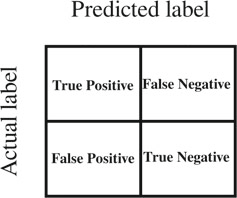
\includegraphics[width=0.3\textwidth]{Images/2-matriz-confusion-binario.png}
    \end{center}
    \caption{Matriz de confusión de un problema de clasificación binario.}
    \reference{Datos tomados de \citeA{aghdam2017guide}.}
    \label{fig:MatrizConfusionBinario}
\end{figure}

La matriz crecerá dependiendo del número de clases a evaluar, la Figura~\ref{fig:MatrizConfusion} muestra una matriz de confusión $5 \times 5 $, este tipo de matrices son utilizadas en tareas de clasificación múltiple o de clasificación multiclase.

\begin{figure}[H]
    \begin{center}
        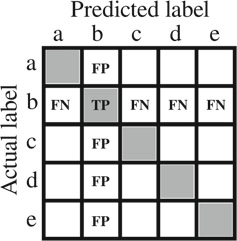
\includegraphics[width=0.3\textwidth]{Images/2-matriz-confusion.png}
    \end{center}
    \caption{Matriz de confusión de un problema de clasificación multiclase.}
    \reference{Datos tomados de \citeA{aghdam2017guide}.}
    \label{fig:MatrizConfusion}
\end{figure}

A partir de la matriz de confusión es posible obtener el valor del accuracy:

\begin{equation}
    accuracy = \frac{TP + TN}{TP + TN + FP + FN}
\end{equation}

Una clasificación perfecta, se da cuando $ FP = FN = 0 $.  El análisis utilizando la matriz de confusión permite determinar el comportamiento del modelo en la practica \cite{aghdam2017guide}.

\textbf{c) Precision y Recall}

Según \citeA{aghdam2017guide}, el precision calcula la fracción de positivos pronosticados y el recall calcula la fracción de positivos reales.

El indicador para el precision está dado por la siguiente ecuación:

\begin{equation}
    precision = \frac{TP}{TP + FP}
\end{equation}

Mientras tanto, la ecuación del recall viene dado por:

\begin{equation}
    recall = \frac{TP}{TP + FN}
\end{equation}

\textbf{d) F1-Score}

Busca determinar una nueva medida para el accuracy del modelo utilizando los indicadores precision y recall \cite{patterson2017deep}. La ecuación del F1-Score está dada por:

\begin{equation}
    F1 = \frac{2}{\frac{1}{precision} + \frac{1}{recall}} = \frac{2 TP}{2TP + FP + FN}
\end{equation}

El valor del indicador está dado por un número entre $ [0,1] $. Si $F1 = 1$ entonces se dice que el modelo es un clasificador perfecto.

\textbf{e) Índice de Jaccard (IoU)}

El Índice de Jaccard, también conocido como Intersect Over Union (IoU), es una métrica comúnmente utilizada en la evaluación de la segmentación de imágenes. Se calcula como la intersección entre la predicción del modelo y la verdad de campo (Ground Truth) dividida por la unión de estas dos áreas. La fórmula para el IoU es:

\begin{equation}
    IoU = \frac{TP}{TP + FP + FN}
\end{equation}

Donde TP es el número de verdaderos positivos, FP es el número de falsos positivos, y FN es el número de falsos negativos. Un valor más alto de IoU indica una mayor precisión en la segmentación \cite{patterson2017deep}.